\documentclass{article}
\usepackage[utf8x]{inputenc}
\usepackage{ucs}
\usepackage{amsmath} 
\usepackage{amsfonts}
\usepackage{upgreek}
\usepackage[english,russian]{babel}
\usepackage{graphicx}
\usepackage{float}
\usepackage{textcomp}
\usepackage{hyperref}
\usepackage{geometry}
  \geometry{left=2cm}
  \geometry{right=1.5cm}
  \geometry{top=1cm}
  \geometry{bottom=2cm}
\usepackage{tikz}
\usepackage{ccaption}
\usepackage{multicol}
\setlength{\columnsep}{1.5cm}
\setlength{\columnseprule}{0.2pt}

\usepackage{listings}


\begin{document}
\pagestyle{plain}
\lstset{
  language=C,                % choose the language of the code
  basicstyle=\linespread{1.1}\ttfamily,
  columns=fixed,
  fontadjust=true,
  basewidth=0.5em,
  keywordstyle=\color{blue}\bfseries,
  commentstyle=\color{gray},
  stringstyle=\ttfamily\color{orange!50!black},
  showstringspaces=false,
  numbersep=5pt,
  numberstyle=\tiny\color{black},
  numberfirstline=true,
  stepnumber=1,                   % the step between two line-numbers.        
  numbersep=10pt,                  % how far the line-numbers are from the code
  backgroundcolor=\color{white},  % choose the background color. You must add \usepackage{color}
  showstringspaces=false,         % underline spaces within strings
  captionpos=b,                   % sets the caption-position to bottom
  breaklines=true,                % sets automatic line breaking
  breakatwhitespace=true,         % sets if automatic breaks should only happen at whitespace
  xleftmargin=.2in,
  extendedchars=\true,
  keepspaces = true,
}
\lstset{literate=%
   *{0}{{{\color{red!20!violet}0}}}1
    {1}{{{\color{red!20!violet}1}}}1
    {2}{{{\color{red!20!violet}2}}}1
    {3}{{{\color{red!20!violet}3}}}1
    {4}{{{\color{red!20!violet}4}}}1
    {5}{{{\color{red!20!violet}5}}}1
    {6}{{{\color{red!20!violet}6}}}1
    {7}{{{\color{red!20!violet}7}}}1
    {8}{{{\color{red!20!violet}8}}}1
    {9}{{{\color{red!20!violet}9}}}1
}

\title{Семинар \#5: Структуры. Классные задачи.\vspace{-5ex}}\date{}\maketitle
\section*{Структуры. Описание, объявление и инициализация:}
Пример программы, в которой описывается структура для удобной работы с объектами Книга (\texttt{Book}).
\begin{lstlisting}
#include <stdio.h>
#include <string.h>

// Создадим новый составной тип под названием struct book
struct book
{
    char title[50];
    int pages;
    float price;
}; // <------------------------ НЕ ЗАБУДЬТЕ ТУТ ТОЧКУ С ЗАПЯТОЙ

void print_book_info(struct book b)
{
    printf("Book info:\n");
    printf("Title: %s\nPages: %d\nPrice: %g\n\n", b.title, b.pages, b.price);
}

int main()
{
    struct book a = {"The Martian", 10, 550.0};
    print_book_info(a);
    a.pages = 369;
    strcpy(a.title, "The Catcher in the Rye");
    print_book_info(a);
    
    struct book scifi_books[10] = {{"Dune", 300, 500.0}, {"Fahrenheit 451", 400, 700.0},
							 {"Day of the Triffids", 304, 450.0}};
    scifi_books[2].price = 2000.0;
    print_book_info(scifi_books[2]);
}
\end{lstlisting}


\subsection*{Задачи:}
\begin{enumerate}
\item \textbf{Структура Дата:} Описать структуру \texttt{struct date}, с полями: \texttt{day}, \texttt{month} и \texttt{year}. 
\begin{itemize}
\item Объявить и инициализировать переменную \texttt{a} даты в функции \texttt{main}.
\item Объявить и инициализировать массив дат под названием \texttt{holidays} следующими значениями \texttt{31.12.2019}, \texttt{8.3.2020} и \texttt{9.5.2020}.
\item Написать функцию \texttt{void print\_date(struct date x)} для печати этой структуры в формате DD.MM.YYYY. Используйте модификатор \texttt{\%02d}. Вызовите эту функцию из main, чтобы напечатать все элементы массива \texttt{holidays}.
\iffalse
\item Написать функцию \texttt{void scan\_date(struct date* px)} для считывания этой структуры в формате DD.MM.YYYY. Вызовите эту функцию из main, чтобы считать переменную \texttt{a} из стандартного входа. Напечатайте эту переменную с помощью \texttt{print\_date}.
\fi
\item Используйте \texttt{typedef}, чтобы сделать имя типа короче. 
\begin{lstlisting}
typedef struct date Date;
\end{lstlisting}
Измените все имена типов с \texttt{struct date} на \texttt{Date}.
\end{itemize}

\item \textbf{Структура Фильм:}
\begin{itemize}
\item \textbf{Описание структуры:} Описать структуру \texttt{Movie} с полями: 
\begin{itemize}
\item \texttt{title} -- название фильма
\item \texttt{running\_time} -- длительность в минутах
\item \texttt{rating} -- оценка на Кинопоиске
\item \texttt{release\_date} -- дата выхода (используйте структуру \texttt{Date}).
\end{itemize}
\item \textbf{Инициализация структуры:} Объявить переменную типа \texttt{Movie} в функции \texttt{main} и инициализировать её следующими значениями:\\
\texttt{title -- ``Joker'', running\_time -- 122, rating -- 7.98, release\_date -- \{3, 10, 2019\}}.
\item \textbf{Доступ с полю структуры:} В новой строке изменить рейтинг и месяц выхода фильма. Используйте оператор точка (\texttt{.}).
\item \textbf{Печать:} Написать функцию \texttt{print\_movie(Movie m)} и вызвать её в функции \texttt{ main()}.
\item \textbf{Массив структур:} Объявить и инициализировать массив, содержащий 10 различных фильмов.
\item \textbf{Печать массива структур:} Написать функцию \texttt{print\_movie\_array(Movie* movies, int n)}, который бы печатал массив структур \texttt{Movie} и вызвать её в функции \texttt{main()}.
\item \textbf{Средний рейтинг:} Написать функцию, которая по массиву фильмов находит средний рейтинг.
\end{itemize}
\end{enumerate}


\section*{Указатели на структуры:}

\begin{lstlisting}
#include <stdio.h>
#include <string.h>
struct book
{
    char title[50];
    int pages;
    float price;
};
typedef struct book Book;

void change_price(Book* p, float new_price) // Передача по указателю
{
	(*p).price = new_price;
}

void print_book_info(const Book* p) // Передача по константному указателю
{
    printf("Book info:\n");
    printf("Title: %s\nPages: %d\nPrice: %g\n\n", p->title, p->pages, p->price);
}

int main()
{
    Book a = {"The Martian", 100, 550.0};
    Book* p = &a;
    
    (*p).pages += 10;
    p->price = 400.0;
    strcpy(p->title, "The Catcher in the Rye");
    change_price(&a, 700);
    print_book_info(&a);
}
\end{lstlisting}

\section*{Указатели на структуры. Задачи:}

\begin{center}
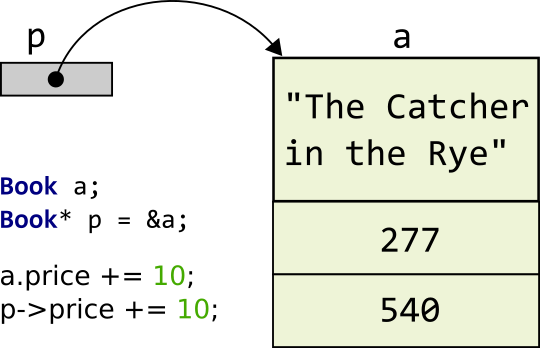
\includegraphics[scale=0.7]{../images/structpointer.png}
\end{center}
\begin{itemize}
\item \textbf{Указатель на структуру:} Создать указатель \texttt{Movie*} и присвоить ему адрес переменной типа \texttt{Movie}.  Изменить поле running\_time, используя только указатель.  Используйте либо оператор точка (\texttt{.}) либо оператор стрелочка (\texttt{->}).
\item \textbf{Передача по адресу:} Написать функцию \texttt{change\_rating(Movie* pm, float new\_rating)} и вызвать её в функции \texttt{main}.
\item \textbf{Считывание:} Написать функцию \texttt{scan\_movie(Movie* m)} и вызвать её в функции \texttt{main}. Функция

\item \textbf{Поиск лучшего фильма:} Написать функцию, которая принимает на вход массив фильмов и возвращает указатель на фильм с самым высоким рейтингом.
\item \textbf{Сортировка структур:} Одна из простейших сортировок - это сортировка выбором:
\begin{lstlisting}
void selection_sort(int n, int arr[])
{
	for (int j = 0; j < n; j++)
	{
		// Находим индекс минимального элемента на отрезке [j:n-1]
		int min_index = j;
		for (int i = j+1; i < n; i++)
			if (arr[i] < arr[min_index])
				min_index = i;
		
		// Меняем местами элемент номер j и минимальный элемент
		int temp = arr[j];
		arr[j] = arr[min_index];
		arr[min_index] = temp;
	}
}
\end{lstlisting}
Видоизмените эту сортировку так, чтобы она сортировала фильмы по рейтингу (от большего к меньшему).
\item \textbf{Сортировка по алфавиту:} Отсортируйте структуры по их названию в алфавитном порядке. Используйте функцию \texttt{strcmp} из \texttt{string.h}. Функция \texttt{strcmp(a, b)} возращает \texttt{0}, если строки равны, отрицательное число если строка \texttt{a} меньше, чем строка \texttt{b} и положительное число, если строка \texttt{a} больше, чем \texttt{b}. 
\item \textbf{Считывание из файла:} Создайте файл \texttt{movies.txt}, который будет хранить информацию о фильмах. Запишите туда 10 фильмов (используйте текстовый редактор). Разделяйте поля с использованием точки с запятой и считывайте строки с помощью спецификатора \verb|%[^;]|.
Напишите программу, которая будет считывать фильмы из файла, записывать их в массив, сортировать и записывать в новый файл.
\end{itemize}


\section*{Справочная информация по указателям:}
Каждая переменная в языке C хранится где-то в памяти и имеет адрес. Адрес переменной это просто номер первого байта соответствующей области памяти. Чтобы получить адрес переменной нужно перед переменной поставить \&(амперсанд).
Указатель это переменная, которая хранит адреса переменных. Тип указателя такой: <тип переменной>*. Пример:
\begin{lstlisting}
int a = 42;  // Переменная, которая хранит число 42
int* address_of_a = &a; // Указатель, который будет хранить адрес переменной a
\end{lstlisting}
Чтобы доступиться к переменной по указателю нужно поставить символ * перед указателем\\
\texttt{a} и \texttt{*address\_of\_a} это абсолютно одно и то же. \texttt{a  ==  *address\_of\_a}.
\begin{lstlisting}
*address_of_a = *address_of_a + 10;
printf("%d", a);  // Напечатает 52
printf("%d", *address_of_a); // Напечатает 52
\end{lstlisting}
Указатели часто используются чтобы изменять передаваемые значения в функциях:
\begin{multicols}{2}
\begin{lstlisting}
// Неправильно:
void normalize(float x, float y)
{
    float sum = x + y;
    x = x / sum;
    y = y / sum; 
    // Изменятся x и y - копии a и b
}
// ...
float a = 20.0, b = 80.0;
normalize(a, b);
// a и b не изменятся: a=20.0, b=80.0
\end{lstlisting}
\begin{lstlisting}

// Правильно:
void normalize(float* px, float* py)
{
    float sum = *px + *py;
    *px = *px / sum;
    *py = *py / sum; 
    // Изменятся переменные a и b
}
// ...
float a = 20.0, b = 80.0;
normalize(&a, &b);
// a и b изменятся:a=0.2, b=0.8
\end{lstlisting}
\end{multicols}
\section*{Типы передачи в функцию:}
\begin{enumerate}
\item По значению. То что передаётся в функцию копируется. При изменении копий, оригинал не меняется.
\begin{lstlisting}
void func(int a)
\end{lstlisting}
\item По указателю. В функцию копируется адрес переменной. Используя этот адрес, можно изменить оригинал.
\begin{lstlisting}
void func(int* p)
\end{lstlisting}
\item По постоянному указателю. В функцию копируется адрес переменной, но изменять оригинал с помощью этого указателя запрещено. Используется для того чтобы передать в функцию переменую большого размера (например структуру) и если вы не хотите изменять её внутри функции. Помогает избежать лишнего копирования.
\begin{lstlisting}
void func(const int* p)
\end{lstlisting}
\end{enumerate}

\end{document}